% !TeX root = ../../main.tex

\begin{figure}[htbp]\label{fig:ripple1}
  \centering
  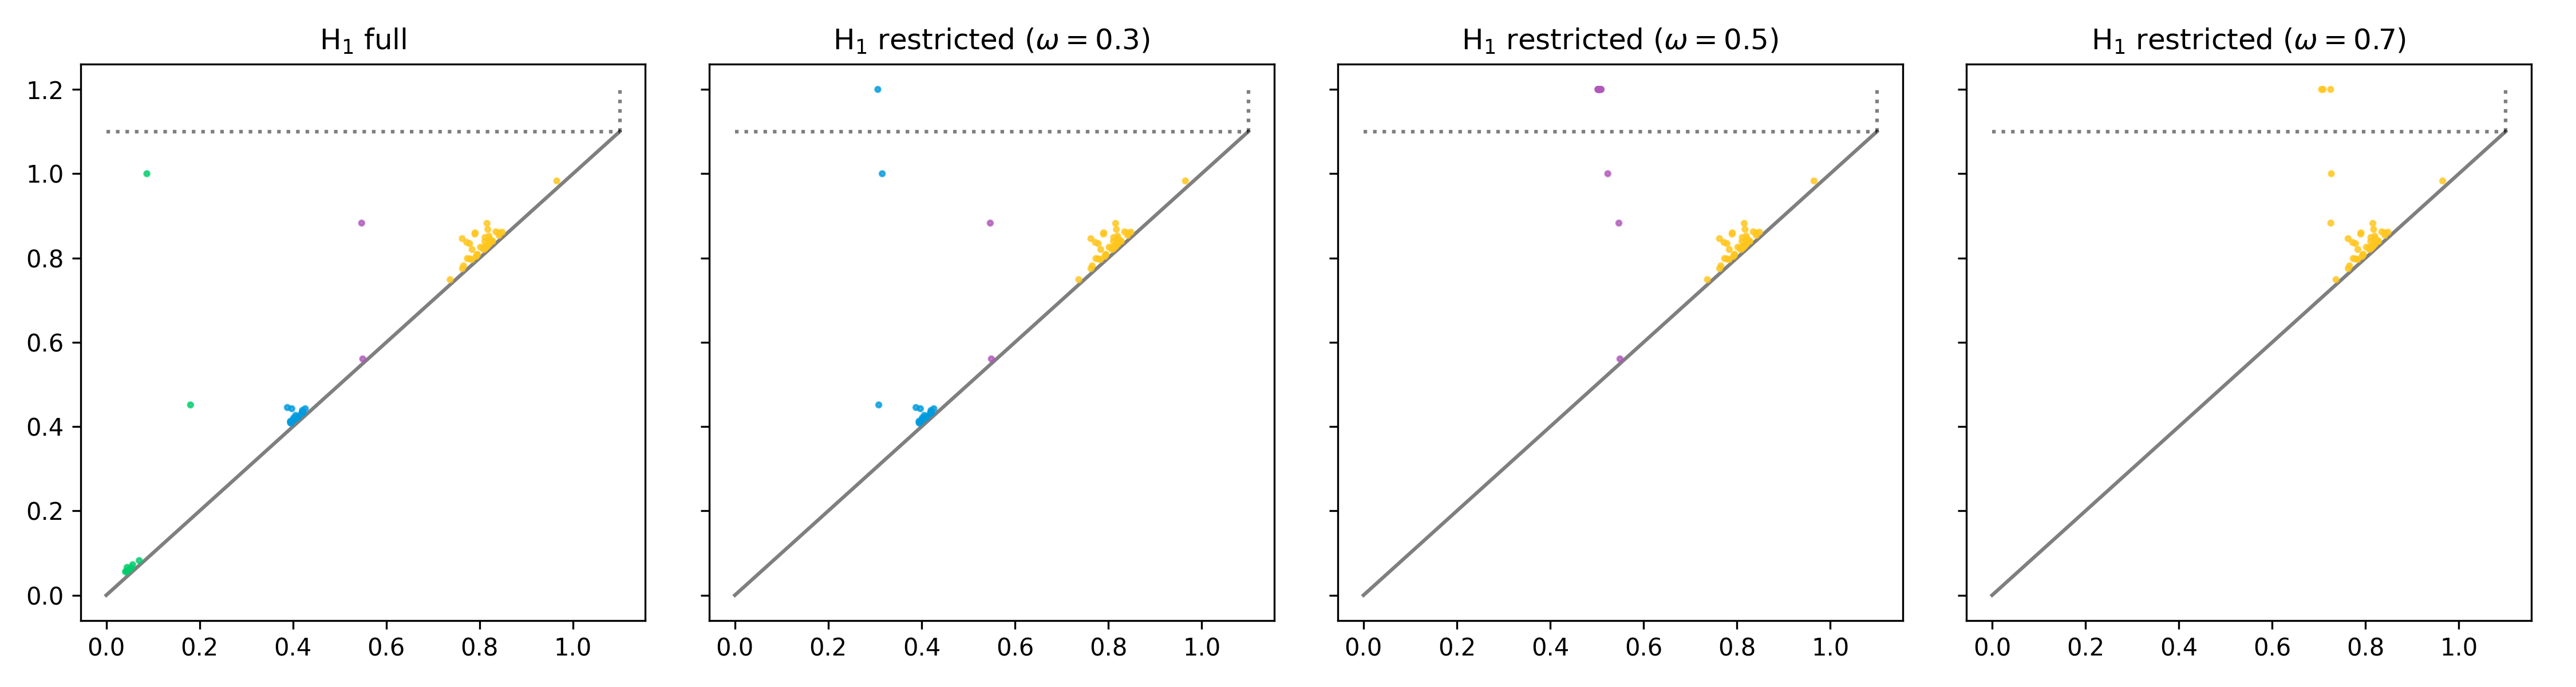
\includegraphics[trim=0 0 790 0, clip, width=0.3\textwidth]{scripts/figures/matching2/full-dgm.png}
  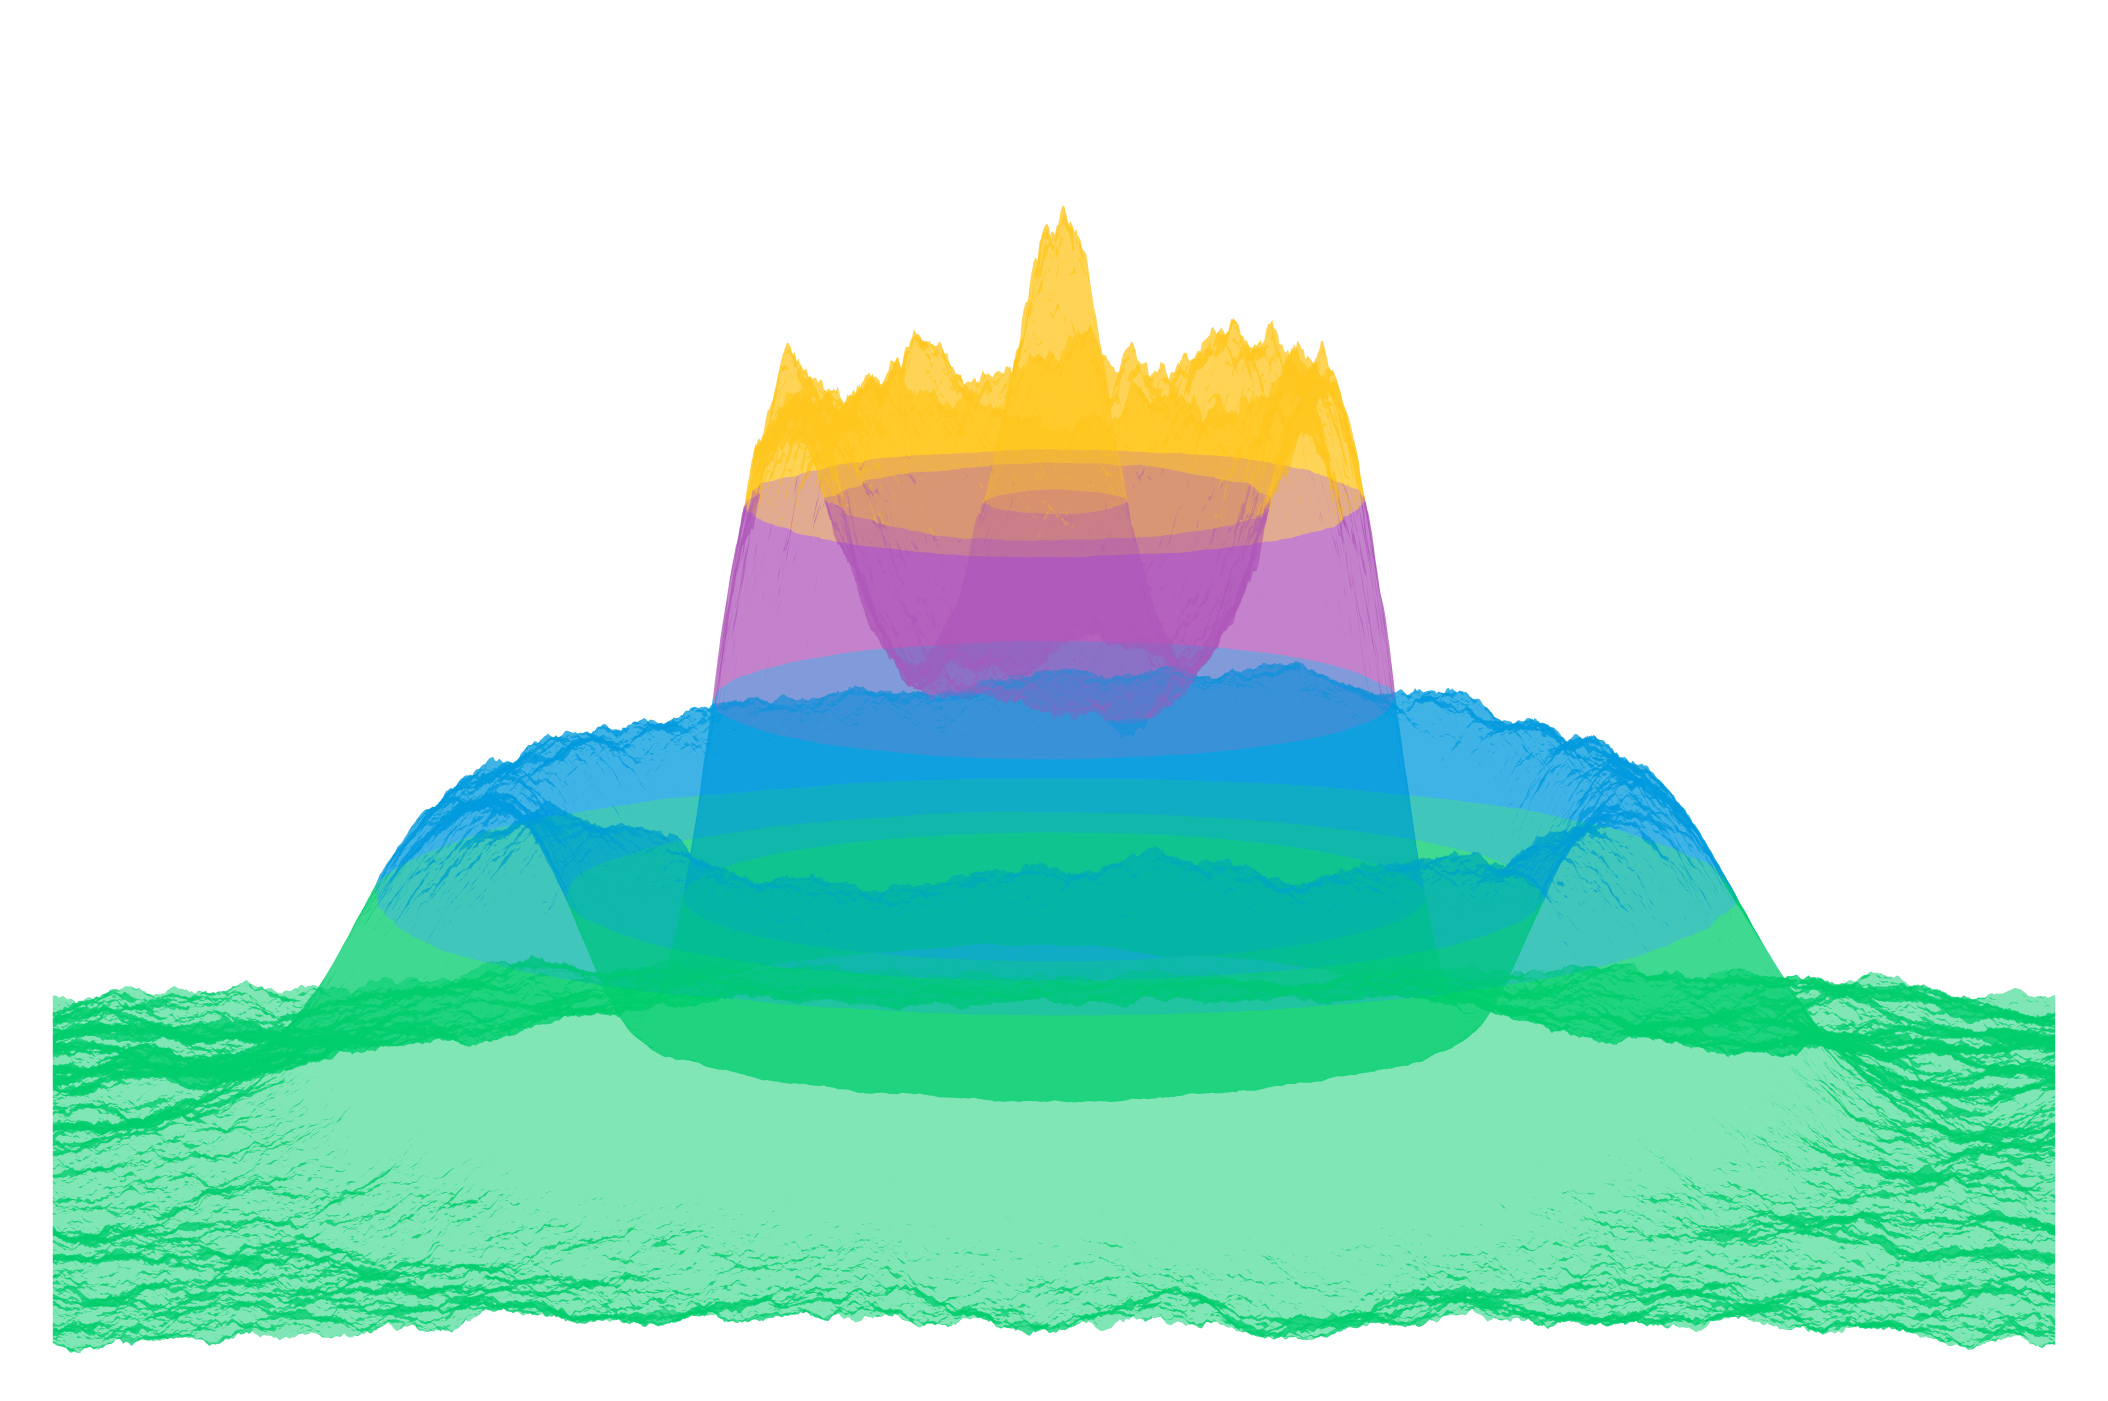
\includegraphics[trim=-350 -800 -700 -300, clip, width=0.4\textwidth]{scripts/figures/matching2/full-surf_side-lowres.png}
  
\includegraphics[trim=0 -800 0 0, width=0.25\textwidth]{scripts/figures/matching2/full-surf_top-lowres.png}
  % \includegraphics[trim=0 0 0 -10, clip, width=\textwidth]{scripts/figures/matching1/817_1024-3_1-1_1.png}
  \caption{The $\hom_1$ persistence diagram of the sinusoidal function pictured to the right.
          Features are colored by birth time, infinite features are drawn above the dotted line.}
\end{figure}

\begin{figure}[htbp]
  \centering
  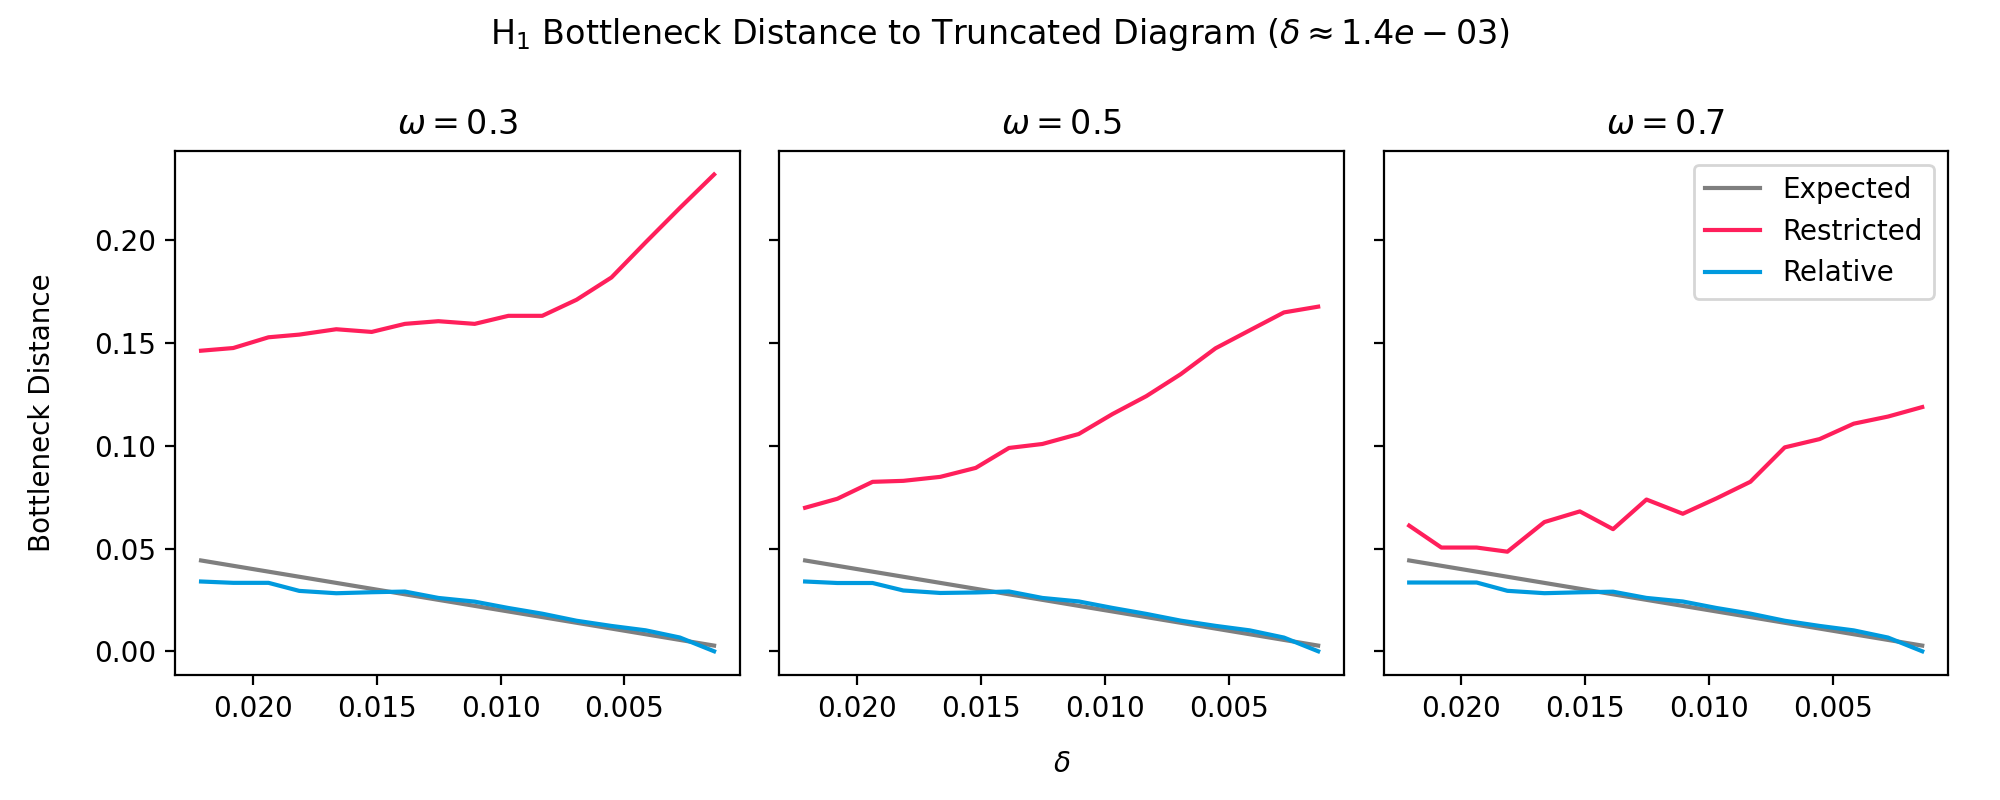
\includegraphics[width=\textwidth]{scripts/figures/matching2/bottleneck_delta.png}
  \caption{Comparison of the bottleneck distance between the truncated diagram of the function shown in Figure~\ref{fig:ripple1} approximated with $\delta\approx 1.4\times10^{-3}$ ($1024\times 1024$ grid) and those of the restricted and relative diagrams with decreasing $\delta$ (increasing grid size 64-1024).}
\end{figure}

\begin{figure}[htbp]
  \centering
  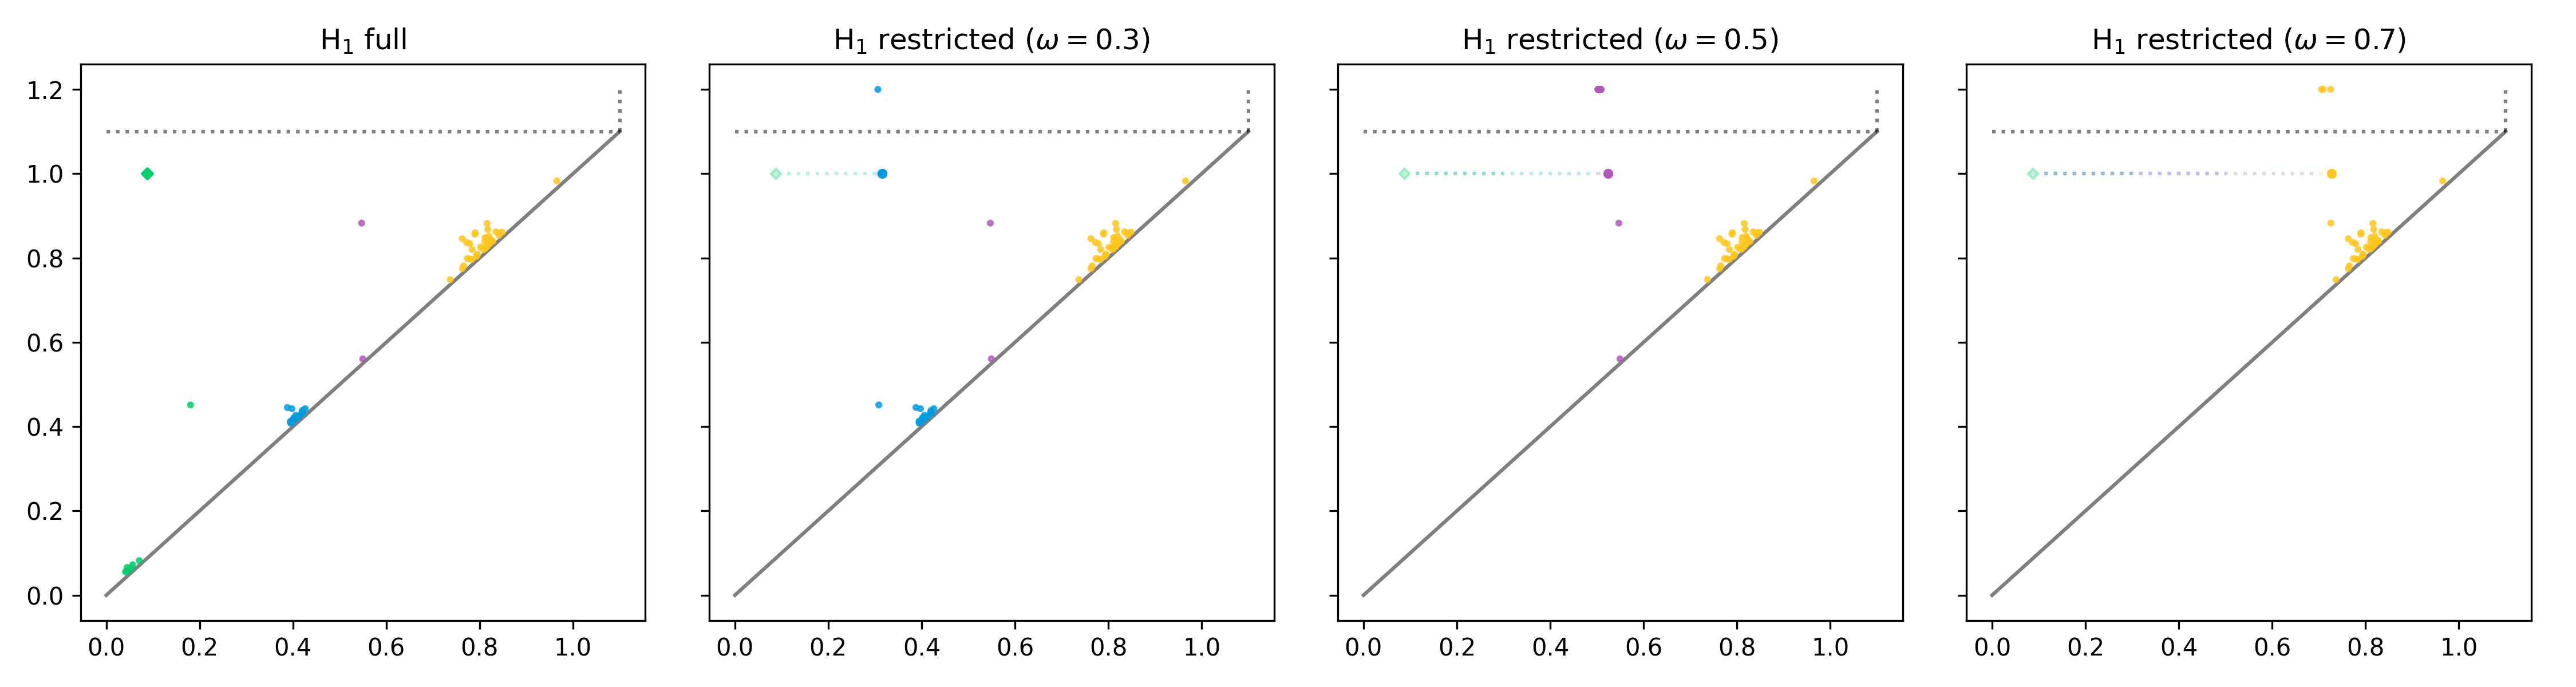
\includegraphics[trim=0 0 -10 0, clip, width=\textwidth]{scripts/figures/matching2/dgm-1.png}
  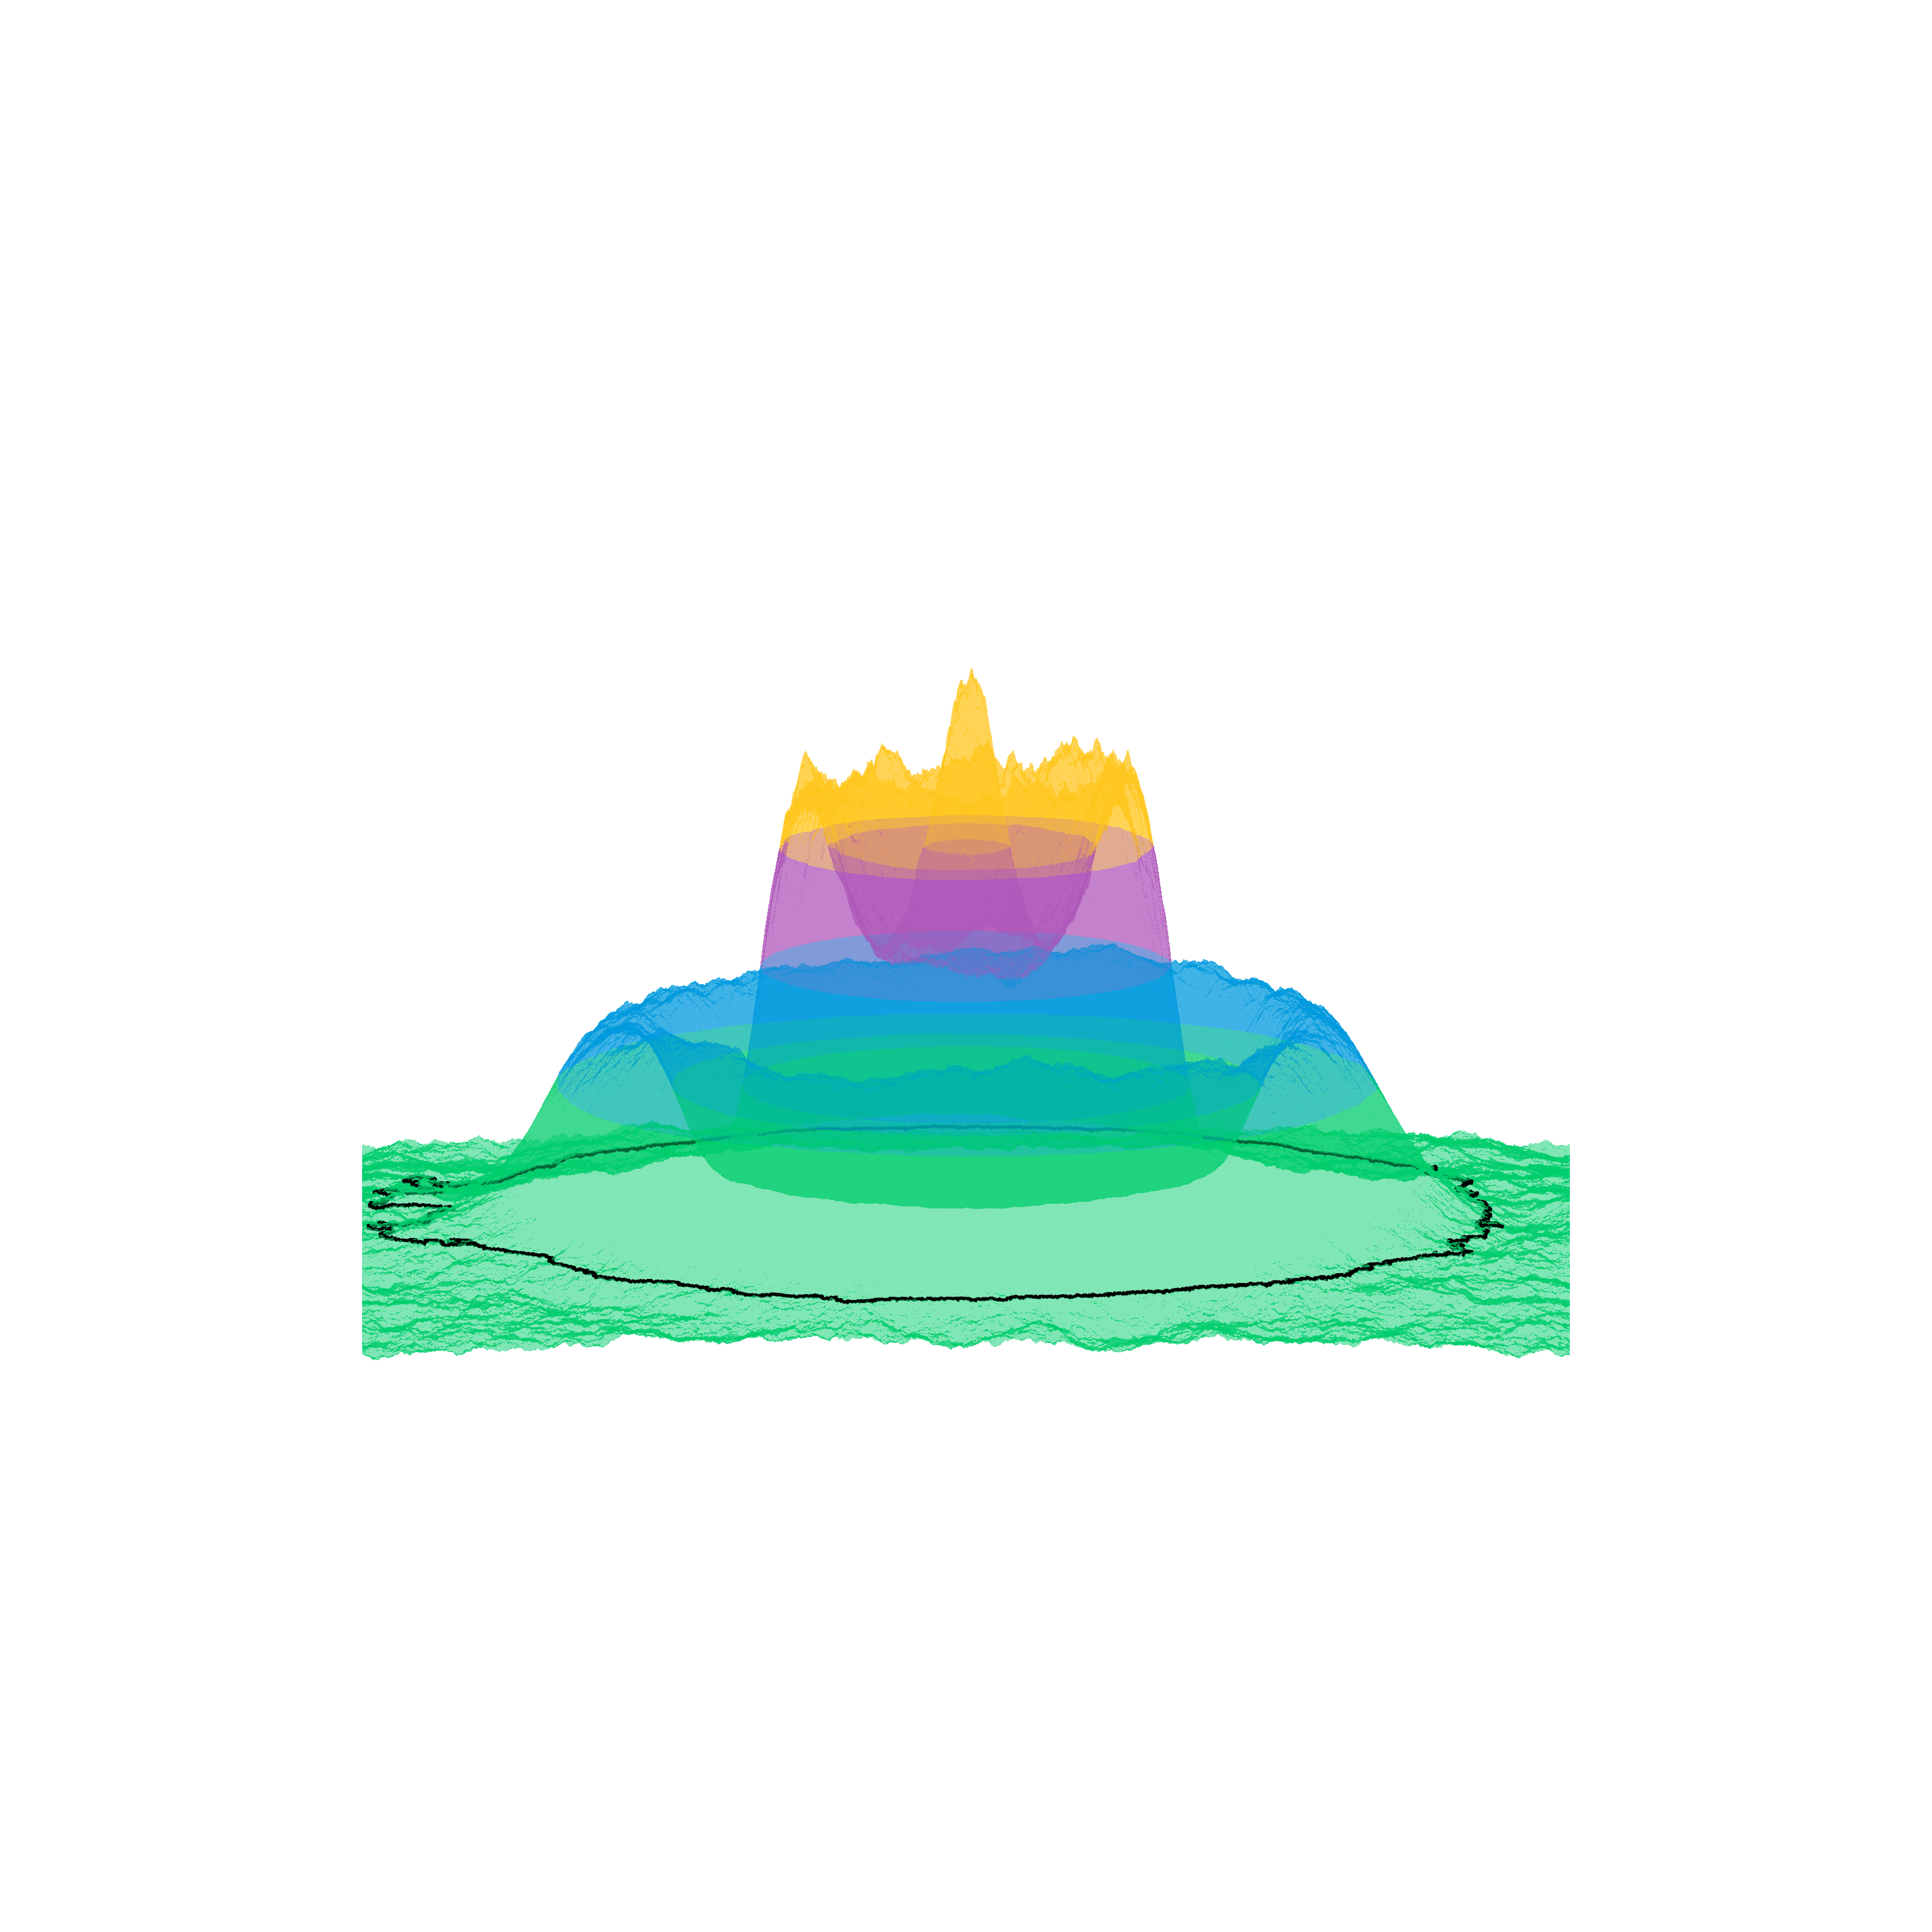
\includegraphics[trim=500 800 500 800, clip, width=0.24\textwidth]{scripts/figures/matching2/surf_side-1.png}
  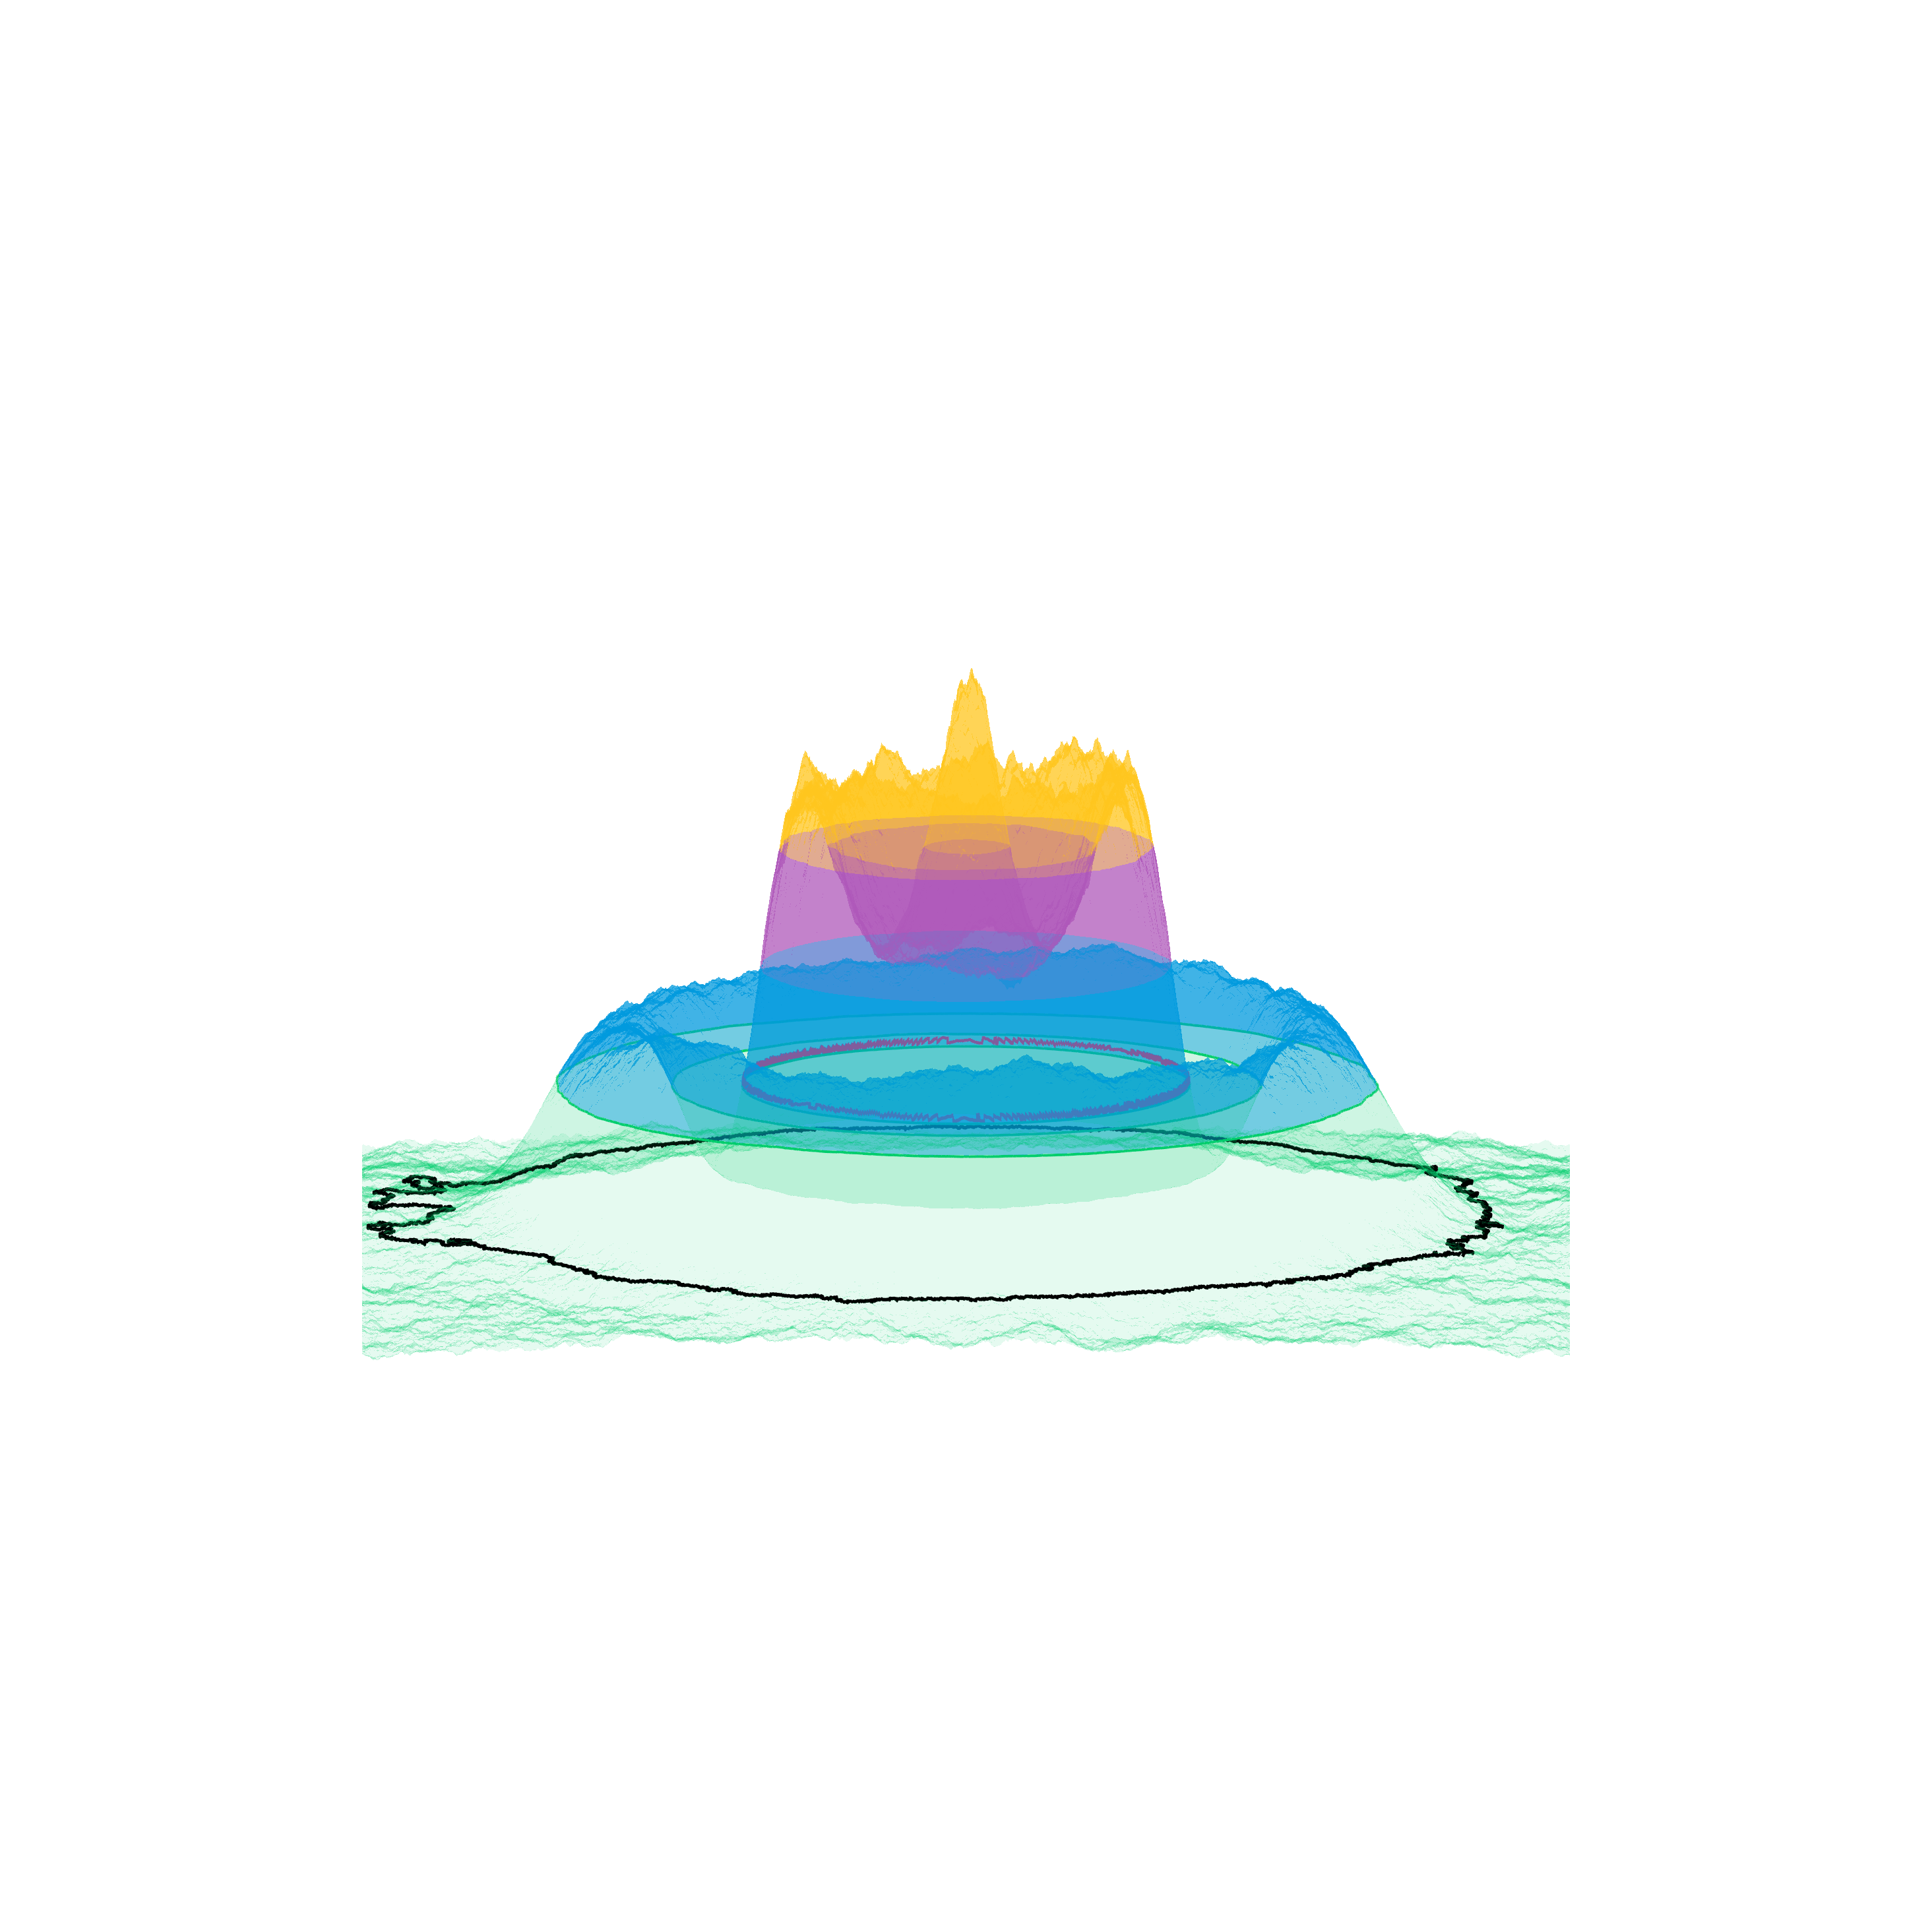
\includegraphics[trim=500 800 500 800, clip, width=0.24\textwidth]{scripts/figures/matching2/surf_side-1_0.png}
  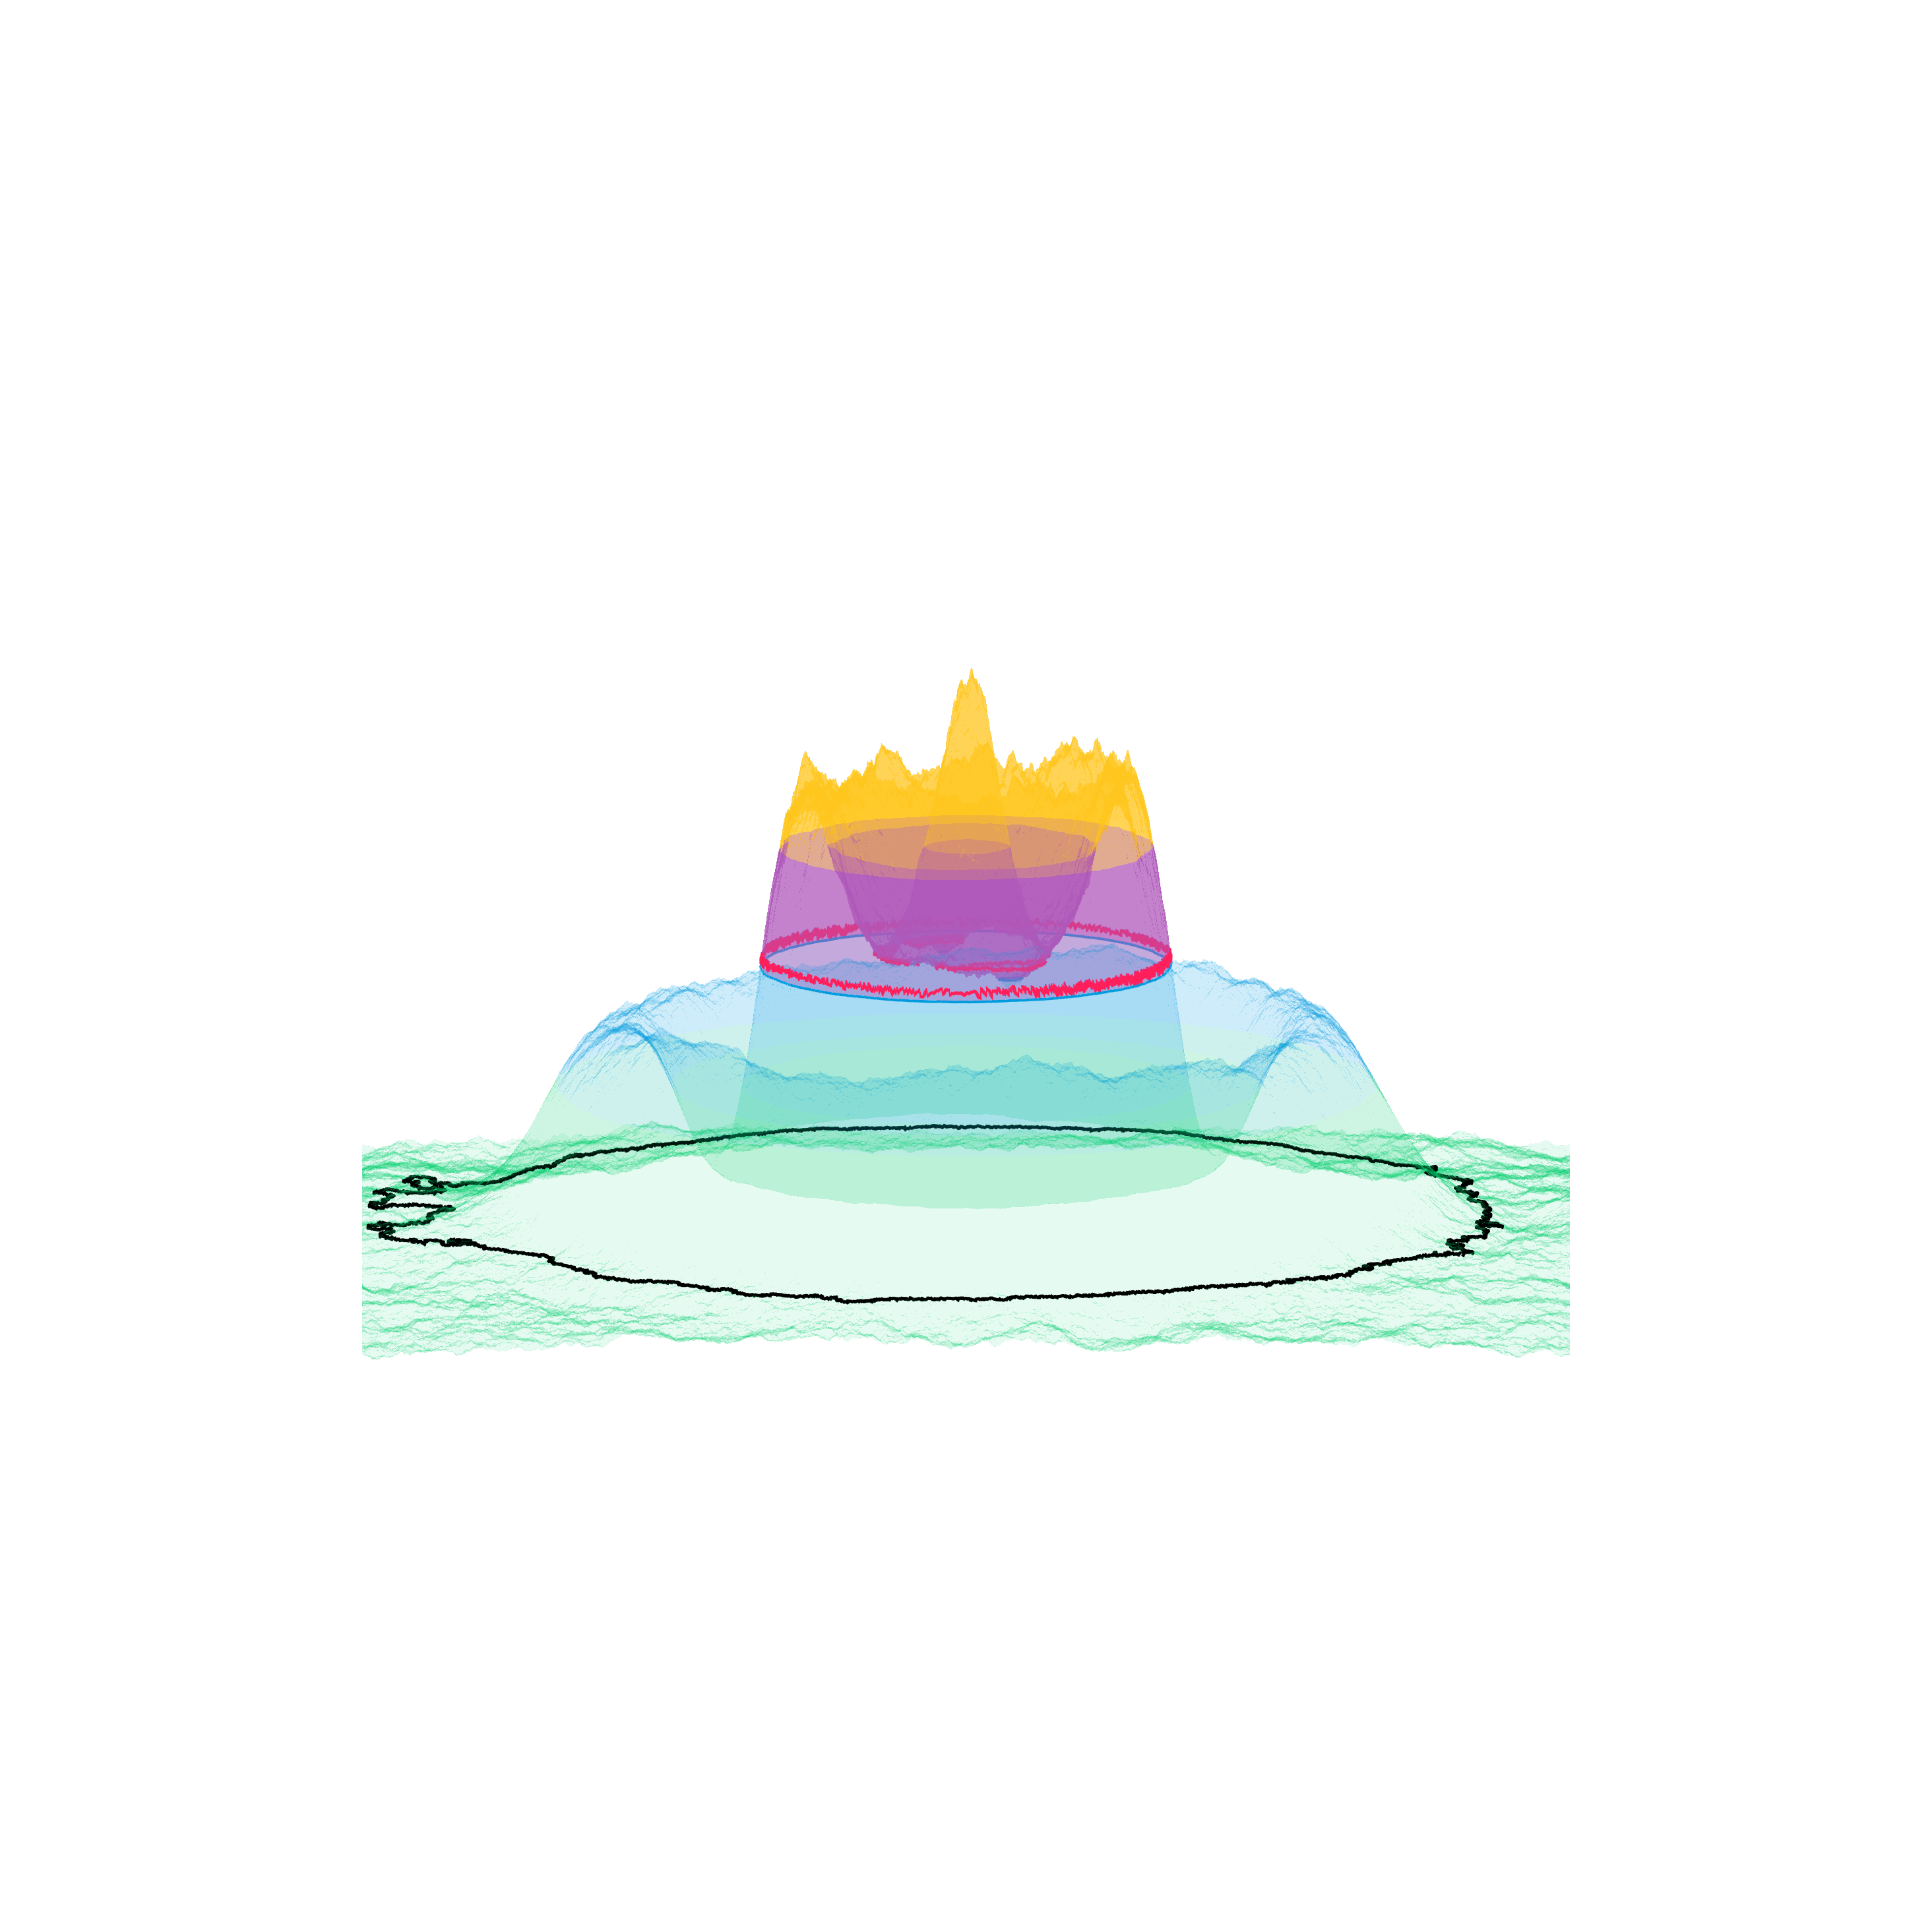
\includegraphics[trim=500 800 500 800, clip, width=0.24\textwidth]{scripts/figures/matching2/surf_side-1_1.png}
  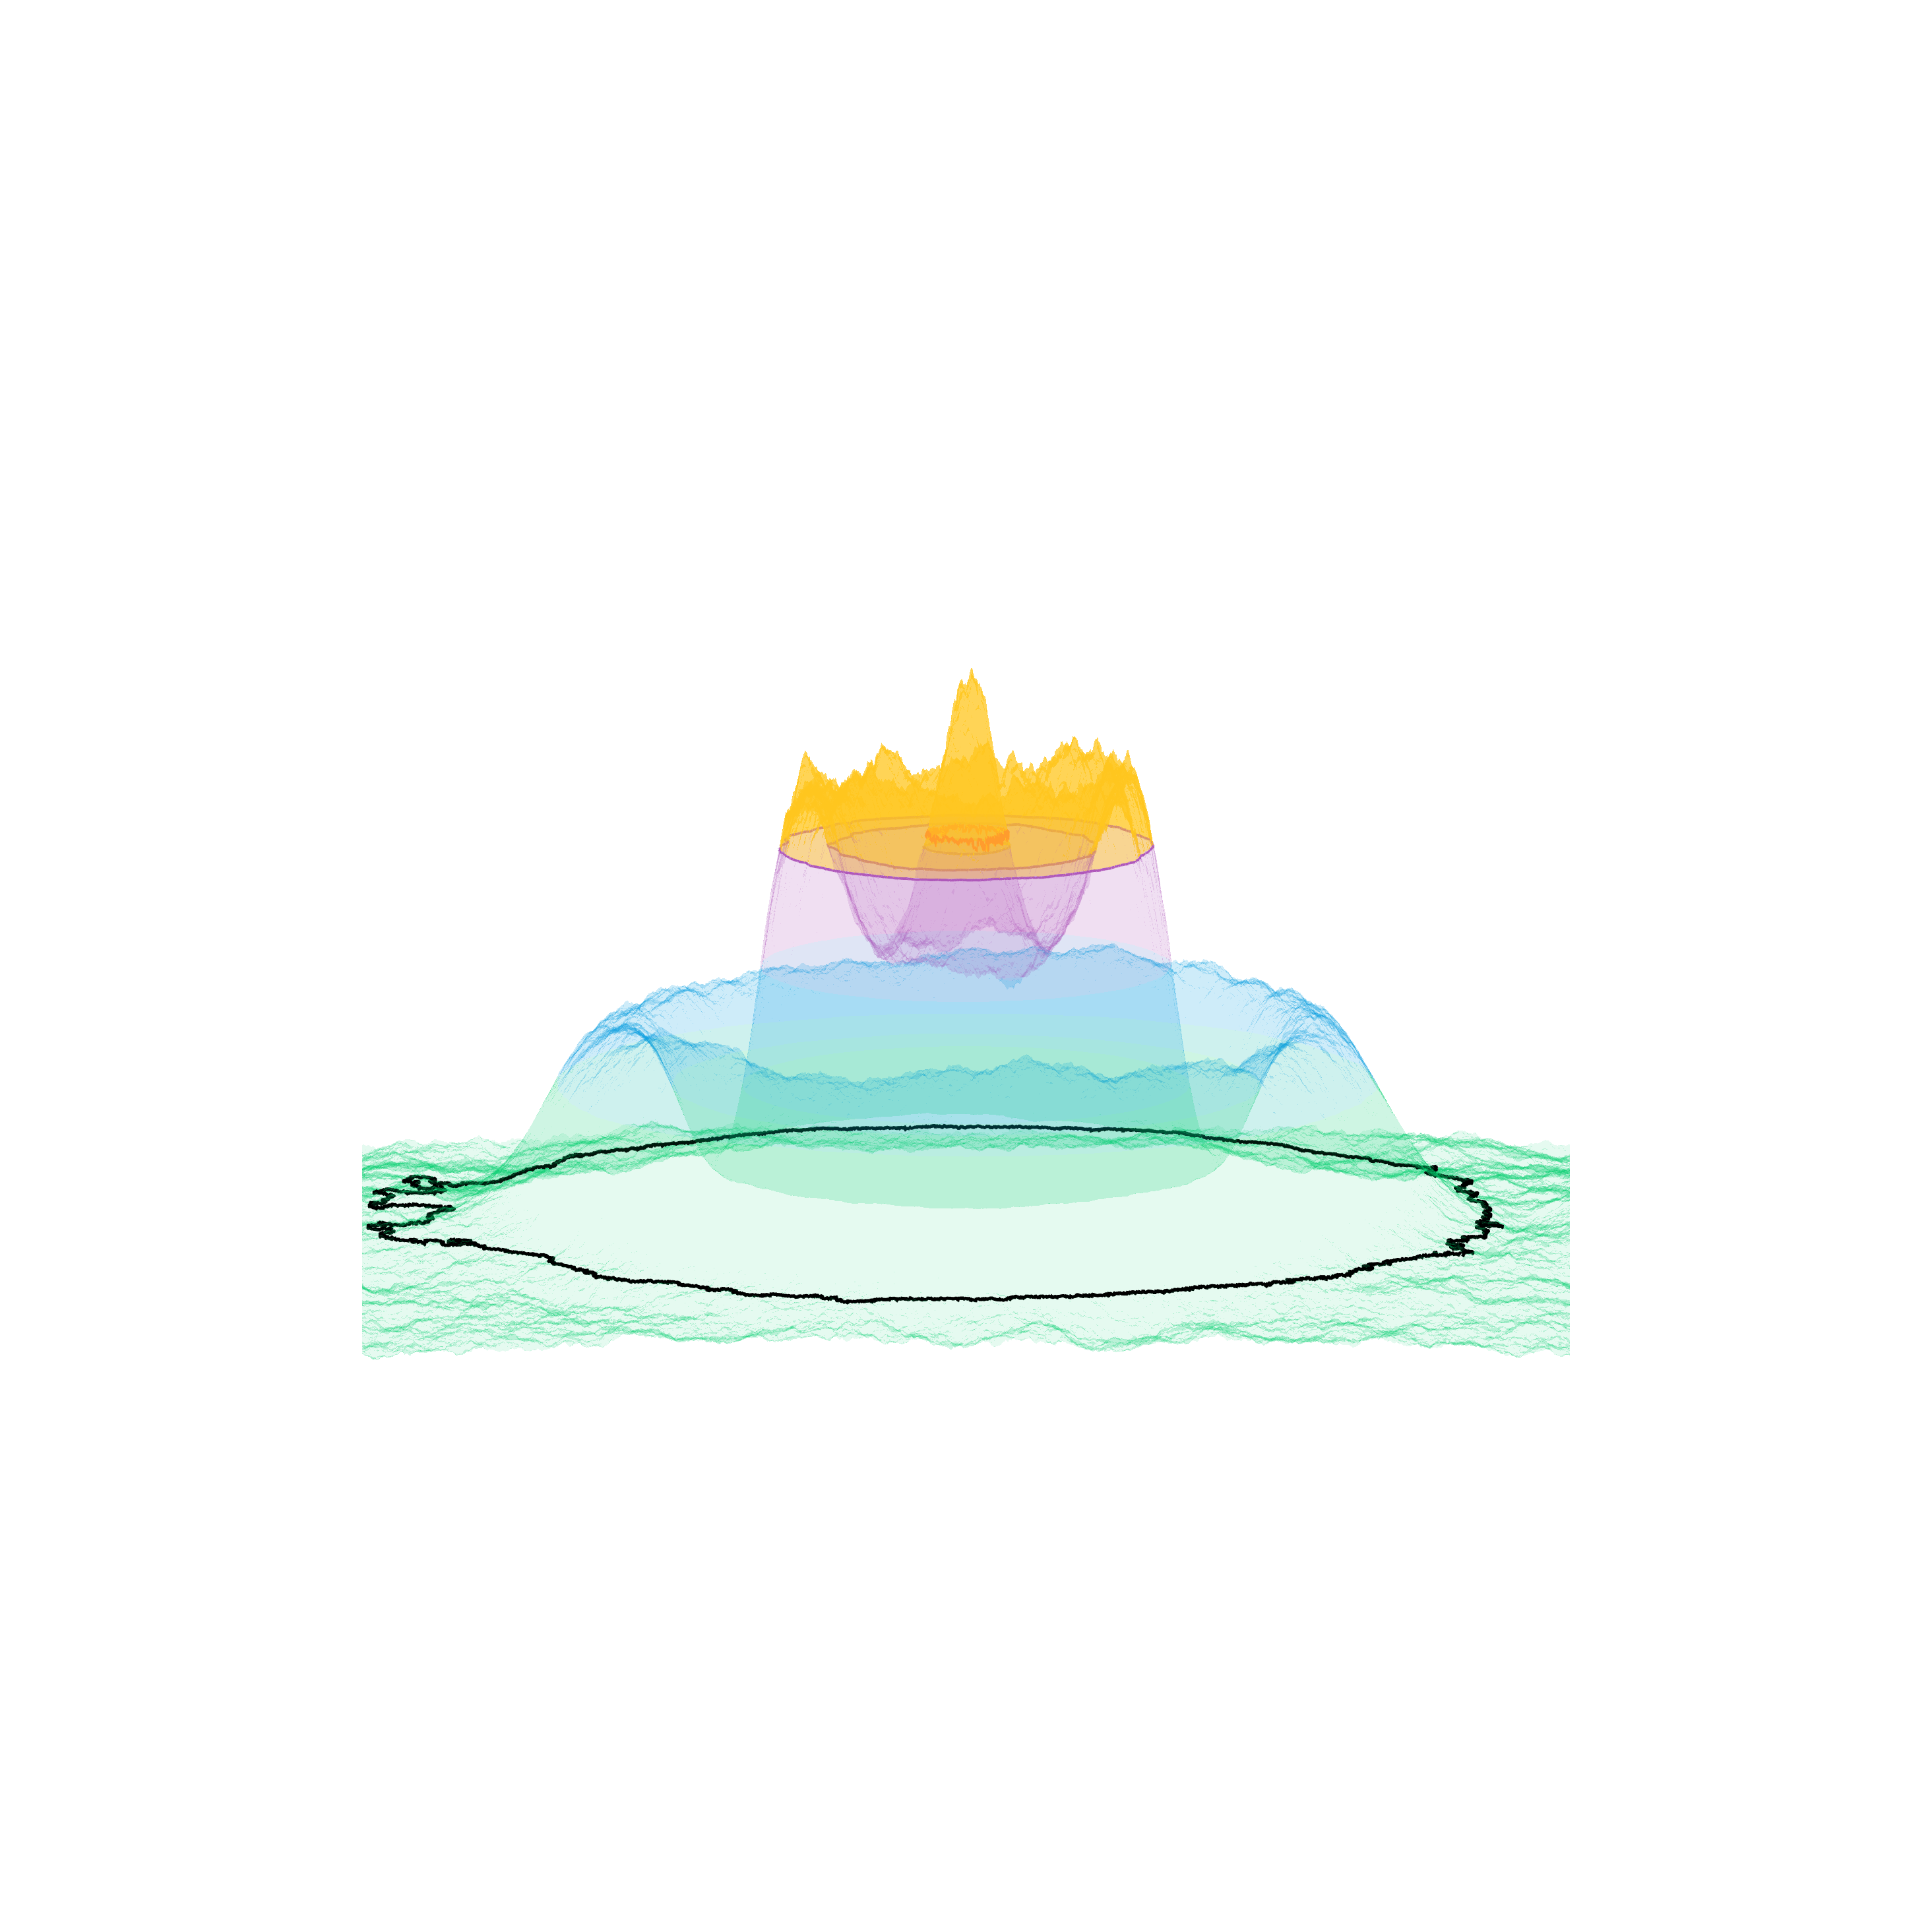
\includegraphics[trim=500 800 500 800, clip, width=0.24\textwidth]{scripts/figures/matching2/surf_side-1_2.png}
  
\includegraphics[trim=500 500 500 500, clip, width=0.24\textwidth]{scripts/figures/matching2/surf_top-1.png}
  
\includegraphics[trim=500 500 500 500, clip, width=0.24\textwidth]{scripts/figures/matching2/surf_top-1_0.png}
  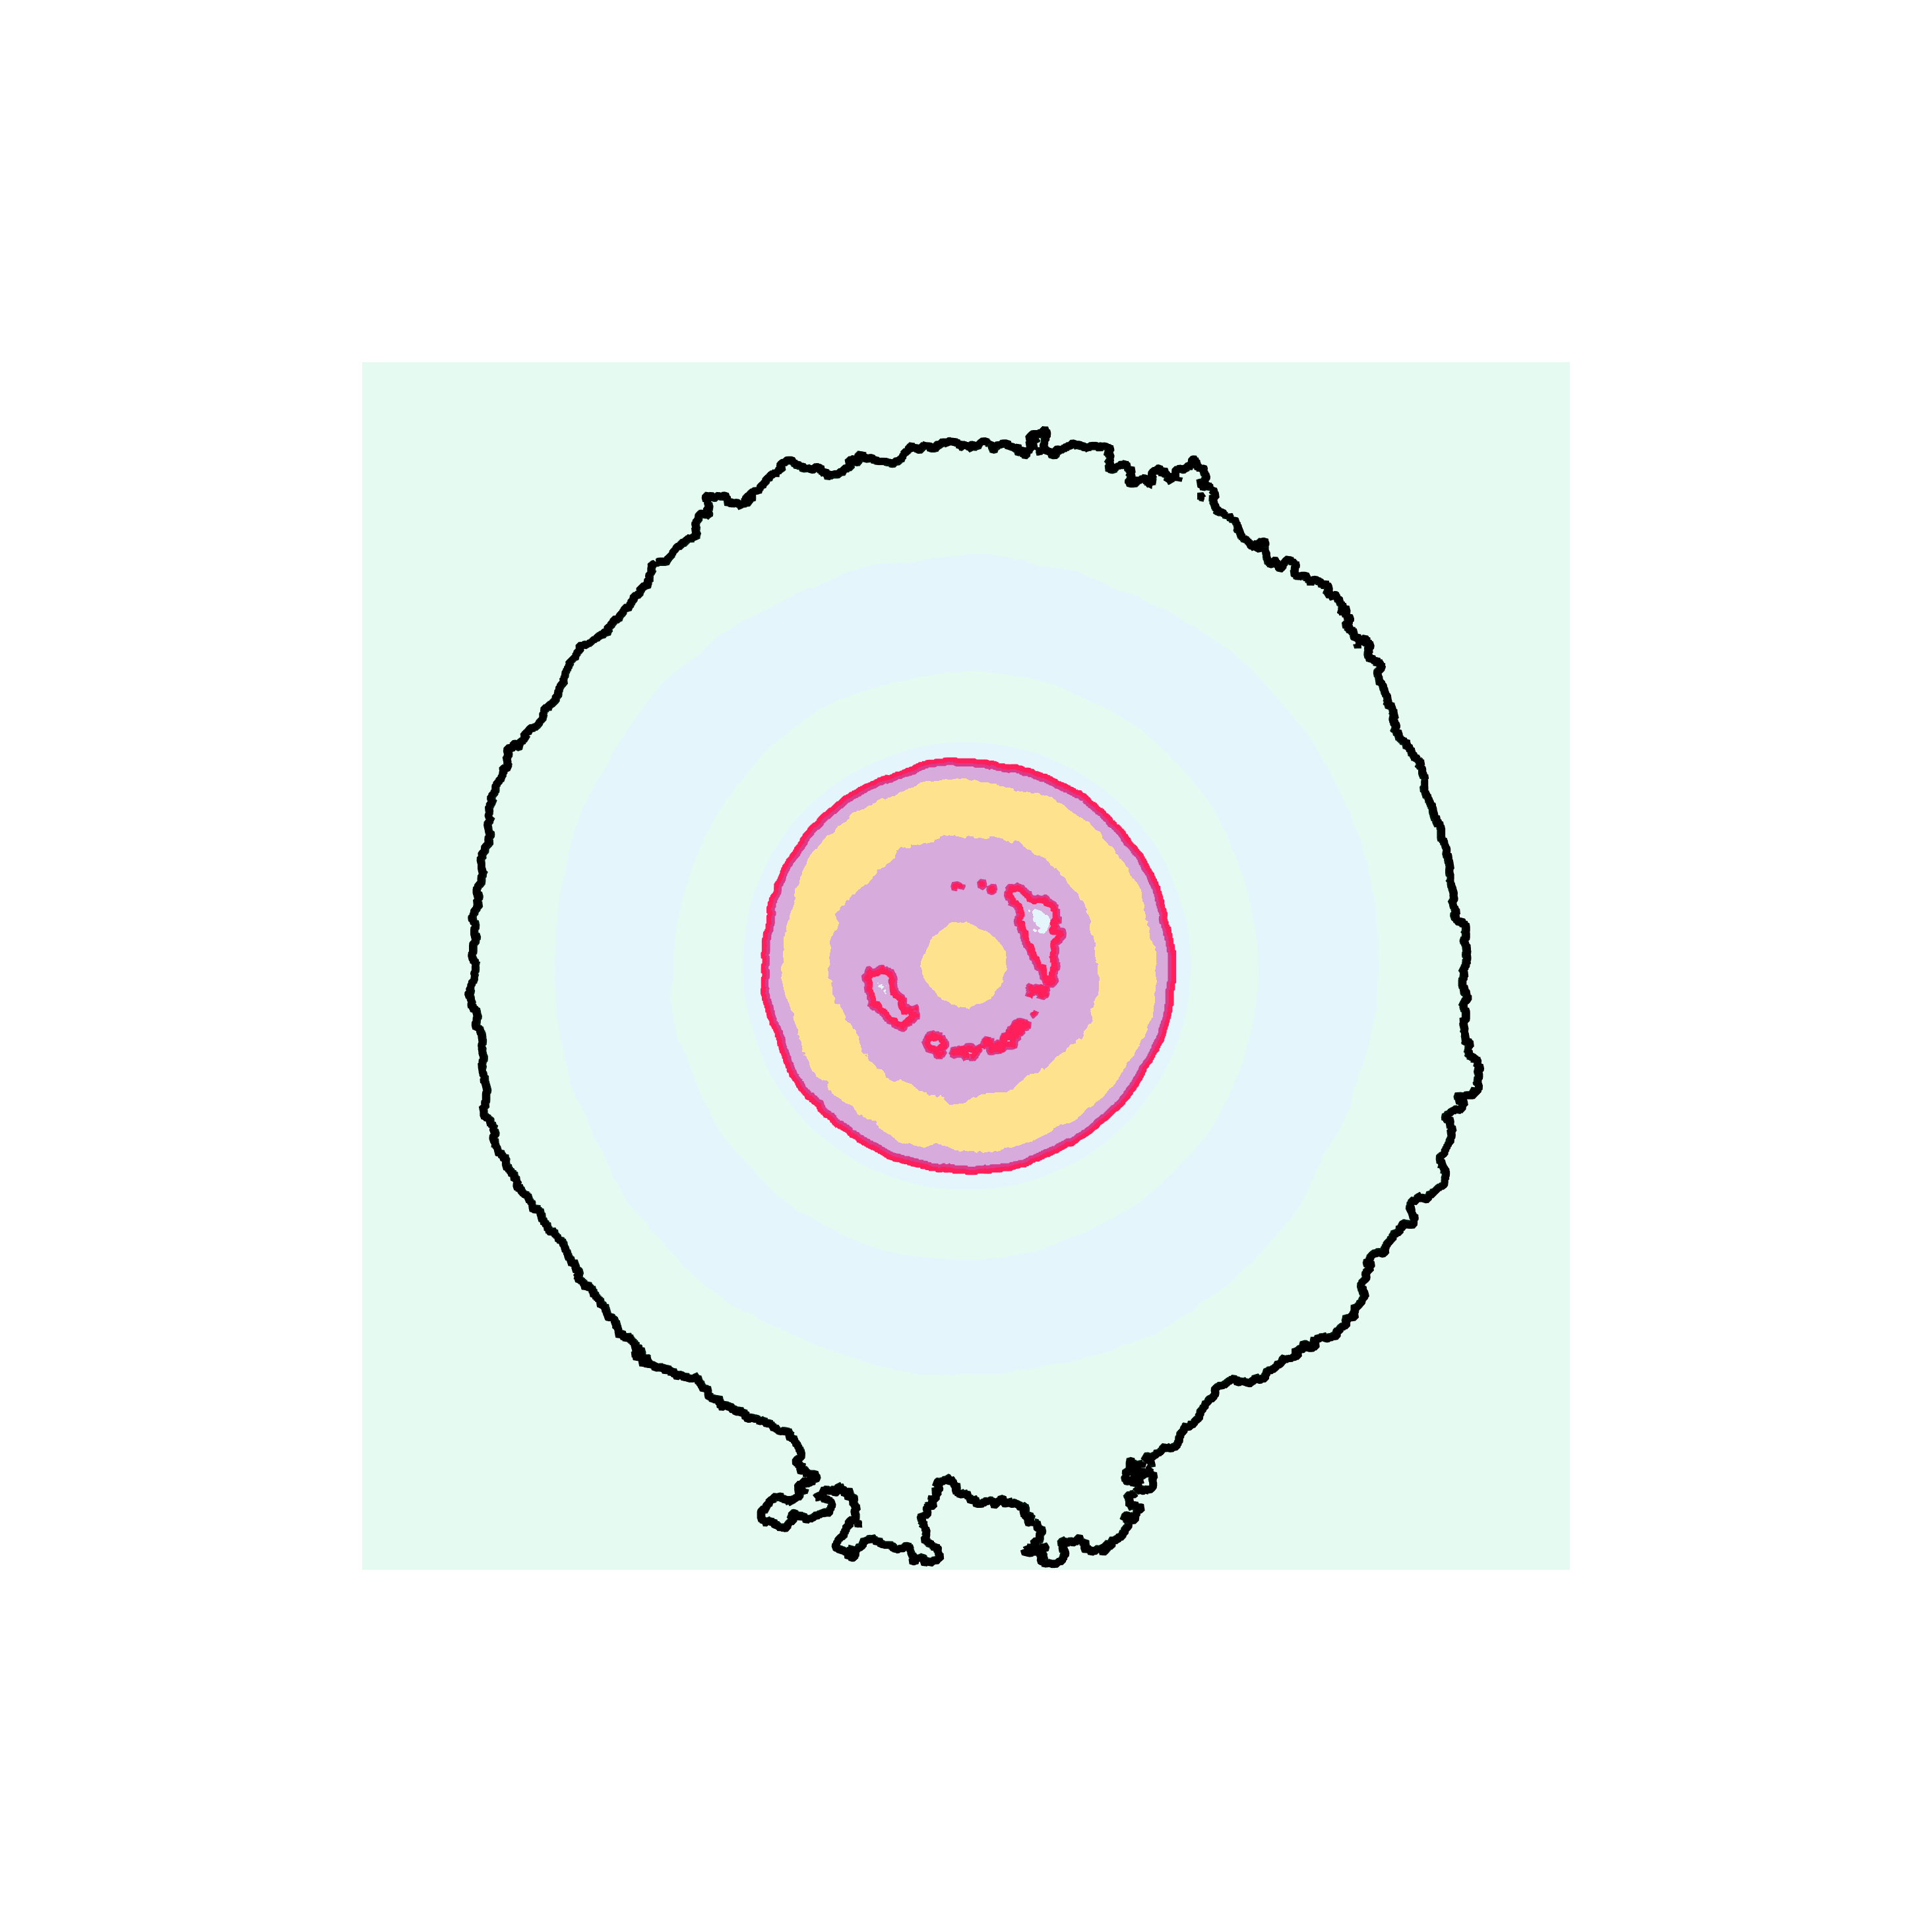
\includegraphics[trim=500 500 500 500, clip, width=0.24\textwidth]{scripts/figures/matching2/surf_top-1_1.png}
  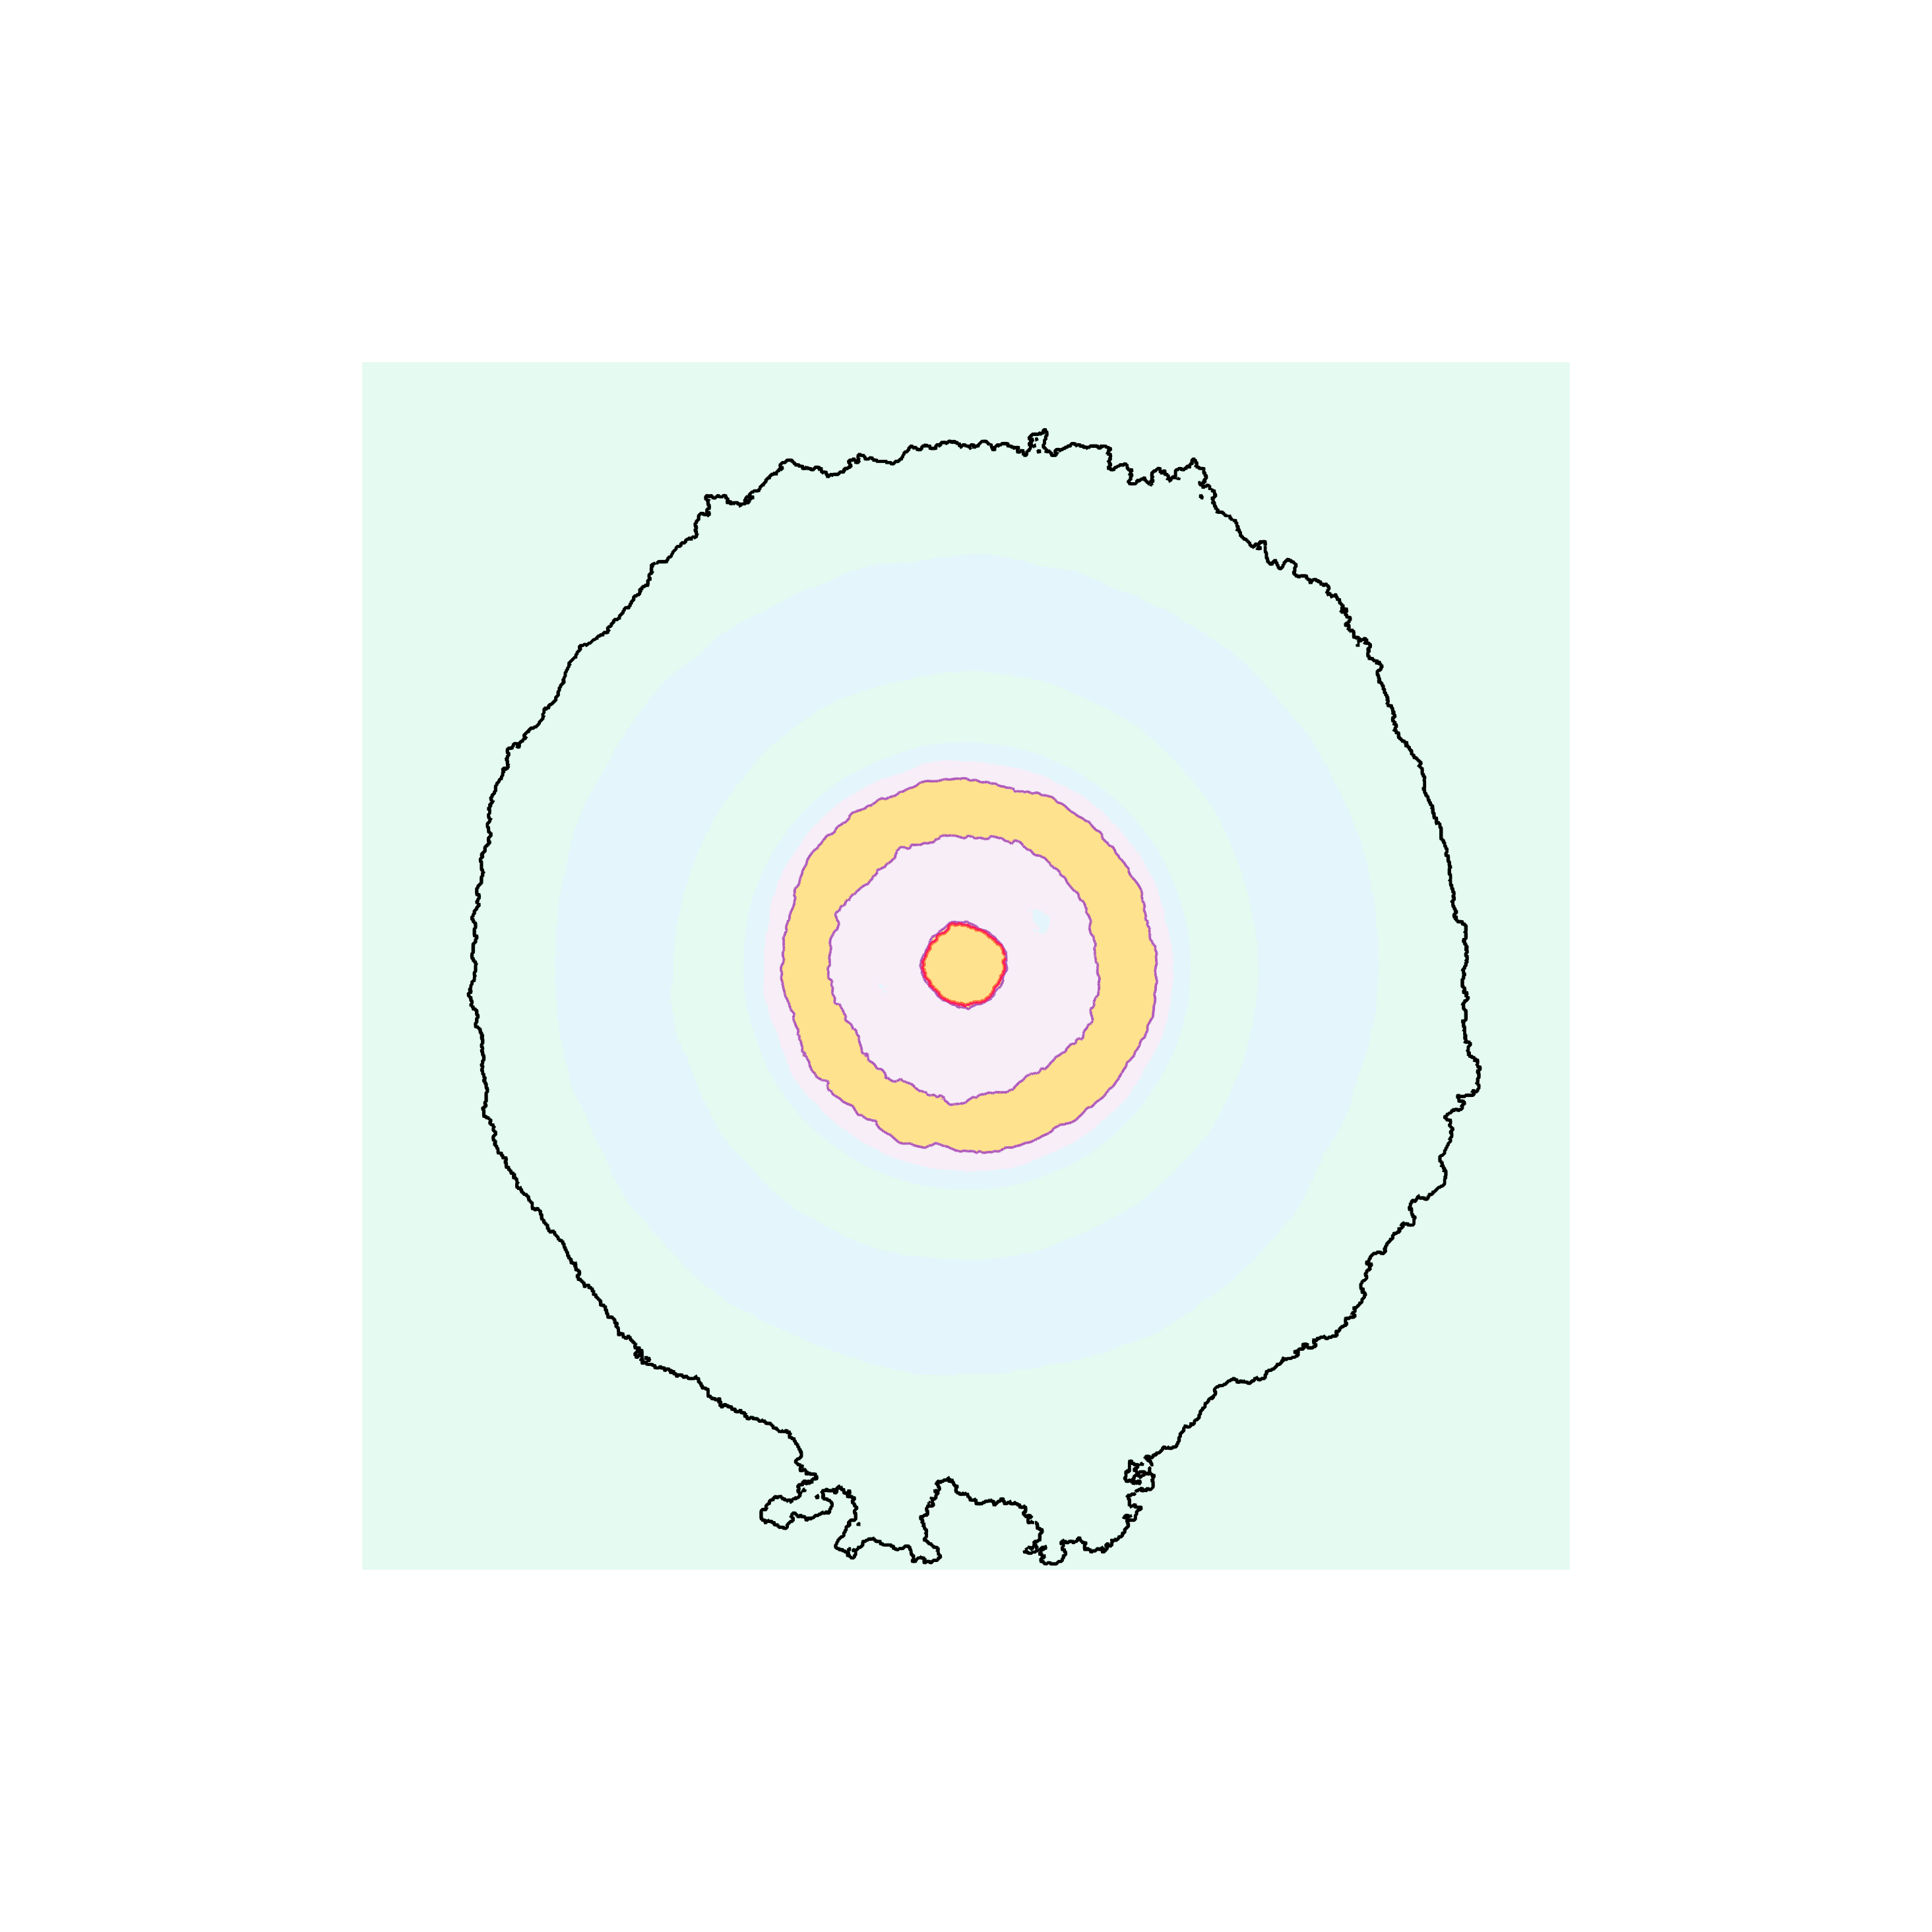
\includegraphics[trim=500 500 500 500, clip, width=0.24\textwidth]{scripts/figures/matching2/surf_top-1_2.png}
  \caption{(Top) $\hom_1$ persistence diagrams of the function depicted in Figure~\ref{fig:ripple1} restricted at $\omega = 0.3, 0.5,$ and $0.7$ (on a $1024\times 1024$ grid).
          The matching is shown between a feature in the full diagram (marked with a diamond) with its representative cycle in black.
          The corresponding representative cycle in the restricted diagram is pictured in red.}
\end{figure}
